\documentclass[a4paper,14pt, unknownkeysallowed]{extreport}

\usepackage{cmap} % Улучшенный поиск русских слов в полученном pdf-файле
\usepackage[T2A]{fontenc} % Поддержка русских букв
\usepackage[utf8]{inputenc} % Кодировка utf8
\usepackage[english,russian]{babel} % Языки: русский, английский
\usepackage{enumitem}


\usepackage{threeparttable}

\usepackage[14pt]{extsizes}

\usepackage{caption}
\captionsetup{labelsep=endash}
\captionsetup[figure]{name={Рисунок}}

% \usepackage{ctable}
% \captionsetup[table]{justification=raggedleft,singlelinecheck=off}

\usepackage{amsmath}

\usepackage{geometry}
\geometry{left=30mm}
\geometry{right=10mm}
\geometry{top=20mm}
\geometry{bottom=20mm}

\usepackage{titlesec}
\titleformat{\section}
	{\normalsize\bfseries}
	{\thesection}
	{1em}{}
\titlespacing*{\chapter}{0pt}{-30pt}{8pt}
\titlespacing*{\section}{\parindent}{*4}{*4}
\titlespacing*{\subsection}{\parindent}{*4}{*4}

\usepackage{setspace}
\onehalfspacing % Полуторный интервал

\frenchspacing
\usepackage{indentfirst} % Красная строка

\usepackage{titlesec}
\titleformat{\chapter}{\LARGE\bfseries}{\thechapter}{20pt}{\LARGE\bfseries}
\titleformat{\section}{\Large\bfseries}{\thesection}{20pt}{\Large\bfseries}

\usepackage{multirow}
\usepackage{listings}
\usepackage{xcolor}

% Для листинга кода:
\lstset{%
	language=python,   					% выбор языка для подсветки	
	basicstyle=\small\sffamily,			% размер и начертание шрифта для подсветки кода
	numbers=left,						% где поставить нумерацию строк (слева\справа)
	numberstyle=\tiny,		   		% размер шрифта для номеров строк
	stepnumber=1,						% размер шага между двумя номерами строк
	numbersep=5pt,						% как далеко отстоят номера строк от подсвечиваемого кода
	frame=single,						% рисовать рамку вокруг кода
	tabsize=4,							% размер табуляции по умолчанию равен 4 пробелам
	captionpos=t,						% позиция заголовка вверху [t] или внизу [b]
	breaklines=true,					
	breakatwhitespace=true,				% переносить строки только если есть пробел
	backgroundcolor=\color{white},
	basicstyle=\footnotesize\ttfamily,
	keywordstyle=\color{blue},
	stringstyle=\color{red},
	commentstyle=\color{gray}
	showspaces=false,
    showstringspaces=false
}


\usepackage{pgfplots}
\usetikzlibrary{datavisualization}
\usetikzlibrary{datavisualization.formats.functions}


\lstset{
	literate=
	{а}{{\selectfont\char224}}1
	{б}{{\selectfont\char225}}1
	{в}{{\selectfont\char226}}1
	{г}{{\selectfont\char227}}1
	{д}{{\selectfont\char228}}1
	{е}{{\selectfont\char229}}1
	{ё}{{\"e}}1
	{ж}{{\selectfont\char230}}1
	{з}{{\selectfont\char231}}1
	{и}{{\selectfont\char232}}1
	{й}{{\selectfont\char233}}1
	{к}{{\selectfont\char234}}1
	{л}{{\selectfont\char235}}1
	{м}{{\selectfont\char236}}1
	{н}{{\selectfont\char237}}1
	{о}{{\selectfont\char238}}1
	{п}{{\selectfont\char239}}1
	{р}{{\selectfont\char240}}1
	{с}{{\selectfont\char241}}1
	{т}{{\selectfont\char242}}1
	{у}{{\selectfont\char243}}1
	{ф}{{\selectfont\char244}}1
	{х}{{\selectfont\char245}}1
	{ц}{{\selectfont\char246}}1
	{ч}{{\selectfont\char247}}1
	{ш}{{\selectfont\char248}}1
	{щ}{{\selectfont\char249}}1
	{ъ}{{\selectfont\char250}}1
	{ы}{{\selectfont\char251}}1
	{ь}{{\selectfont\char252}}1
	{э}{{\selectfont\char253}}1
	{ю}{{\selectfont\char254}}1
	{я}{{\selectfont\char255}}1
	{А}{{\selectfont\char192}}1
	{Б}{{\selectfont\char193}}1
	{В}{{\selectfont\char194}}1
	{Г}{{\selectfont\char195}}1
	{Д}{{\selectfont\char196}}1
	{Е}{{\selectfont\char197}}1
	{Ё}{{\"E}}1
	{Ж}{{\selectfont\char198}}1
	{З}{{\selectfont\char199}}1
	{И}{{\selectfont\char200}}1
	{Й}{{\selectfont\char201}}1
	{К}{{\selectfont\char202}}1
	{Л}{{\selectfont\char203}}1
	{М}{{\selectfont\char204}}1
	{Н}{{\selectfont\char205}}1
	{О}{{\selectfont\char206}}1
	{П}{{\selectfont\char207}}1
	{Р}{{\selectfont\char208}}1
	{С}{{\selectfont\char209}}1
	{Т}{{\selectfont\char210}}1
	{У}{{\selectfont\char211}}1
	{Ф}{{\selectfont\char212}}1
	{Х}{{\selectfont\char213}}1
	{Ц}{{\selectfont\char214}}1
	{Ч}{{\selectfont\char215}}1
	{Ш}{{\selectfont\char216}}1
	{Щ}{{\selectfont\char217}}1
	{Ъ}{{\selectfont\char218}}1
	{Ы}{{\selectfont\char219}}1
	{Ь}{{\selectfont\char220}}1
	{Э}{{\selectfont\char221}}1
	{Ю}{{\selectfont\char222}}1
	{Я}{{\selectfont\char223}}1
}

\usepackage{graphicx}
\newcommand{\img}[3] {
	\begin{figure}[h!]
		\center{\includegraphics[height=#1]{img/#2}}
		\caption{#3}
		\label{img:#2}
	\end{figure}
}


\usepackage[justification=centering]{caption} % Настройка подписей float объектов

\usepackage[unicode,pdftex]{hyperref} % Ссылки в pdf
\hypersetup{hidelinks}

\usepackage{csvsimple}

\newcommand{\code}[1]{\texttt{#1}}

\usepackage{longtable}

\usepackage{array}
\usepackage{booktabs}
\usepackage{floatrow}

\floatsetup[longtable]{LTcapwidth=table}



\begin{document}


\begin{titlepage}
	\newgeometry{pdftex, left=2cm, right=2cm, top=2.5cm, bottom=2.5cm}
	\fontsize{12pt}{12pt}\selectfont
	\noindent \begin{minipage}{0.15\textwidth}
		
\includegraphics[width=\linewidth]{img/b_logo.jpg}
	\end{minipage}
	\noindent\begin{minipage}{0.9\textwidth}\centering
		\textbf{Министерство науки и высшего образования Российской Федерации}\\
		\textbf{Федеральное государственное бюджетное образовательное учреждение высшего образования}\\
		\textbf{«Московский государственный технический университет имени Н. Э.~Баумана}\\
		\textbf{(национальный исследовательский университет)»}\\
		\textbf{(МГТУ им. Н. Э.~Баумана)}
	\end{minipage}
	
	\noindent\rule{18cm}{3pt}
	\newline\newline
	\noindent ФАКУЛЬТЕТ $\underline{\text{«Информатика и системы управления»~~~~~~~~~~~~~~~~~~~~~~~~~~~~~~~~~~~~~~~~~~~~~~~~~~~~~~~}}$ \newline\newline
	\noindent КАФЕДРА $\underline{\text{«Программное обеспечение ЭВМ и информационные технологии»~~~~~~~~~~~~~~~~~~~~~~~}}$\newline\newline\newline\newline\newline\newline\newline
	
	
	\begin{center}
		\noindent\begin{minipage}{1.3\textwidth}\centering
		\Large\textbf{   ~~~ Лабораторная работа №6}\newline
		\textbf{по дисциплине "Анализ Алгоритмов"}\newline\newline\newline
		\end{minipage}
	\end{center}
	
	\noindent\textbf{Тема} 			$\underline{\text{Муравьиный алгоритм}}$\newline\newline
	\noindent\textbf{Студент} 		$\underline{\text{Ковалец К. Э.}}$\newline\newline
	\noindent\textbf{Группа} 		$\underline{\text{ИУ7-53Б}}$\newline\newline
	\noindent\textbf{Преподаватель} $\underline{\text{Волкова Л. Л.}}$\newline
	
	\begin{center}
		\vfill
		Москва~---~\the\year
		~г.
	\end{center}
	\restoregeometry
\end{titlepage}



\renewcommand{\contentsname}{Содержание} 
\tableofcontents
\setcounter{page}{2}





\chapter*{Введение}
\addcontentsline{toc}{chapter}{Введение}

Задача поиска оптимальных маршрутов является одной из важных.
Муравьиный алгоритм – один из эффективных полиномиальных алгоритмов для нахождения приближённых решений задачи коммивояжёра, а также решения аналогичных задач поиска маршрутов на графах. Суть подхода заключается в анализе и использовании модели поведения муравьёв, ищущих пути от колонии к источнику питания, и представляет собой метаэвристическую оптимизацию.

Целью данной лабораторной работы является изучение муравьиного алгоритма на примере задачи коммивояжера.

Для достижения поставленной цели необходимо выполнить следующие задачи:

\begin{itemize}
	\item исследовать задачу коммивояжера;
	\item изучить алгоритм полного перебора и муравьиный алгоритм для решения задачи коммивояжера;
	\item провести параметризацию муравьиного алгоритма на двух классах данных;
	\item привести схемы используемых алгоритмов;
	\item описать используемые структуры данных;
	\item описать структуру разрабатываемого ПО;
	\item определить средства программной реализации;
	\item провести сравнительный анализ времени работы алгоритмов;
	\item провести функциональное тестирование;
	\item описать и обосновать полученные результаты в отчете о выполненной лабораторной работе.
\end{itemize}





\chapter{Аналитическая часть}

В данном разделе будет представлено описание задачи коммивояжера и используемых для её решения алгоритмов (полного перебора и муравьиного алгоритма).

\section{Задача коммивояжера}


Коммивояжёр (фр. commis voyageur) — бродячий торговец. Задача коммивояжёра [1] — одна из самых важных задач транспортной логистики, отрасли, занимающейся планированием транспортных перевозок. Коммивояжёру, чтобы распродать товары, следует объехать $n$ пунктов и в конце концов вернуться в исходный пункт. Требуется определить наиболее выгодный маршрут объезда. В качестве меры выгодности маршрута может служить суммарное время в пути, суммарная стоимость дороги, или, в простейшем случае, длина маршрута.

 В описываемой задаче рассматривается несколько городов и матрица попарных расстояний между ними (матрица смежности).


\section{Алгоритм полного перебора}


Алгоритм полного перебора [2] для решения задачи коммивояжера предполагает рассмотрение всех возможных путей в графе и выбор наименьшего из них. Смысл перебора состоит в том, что мы перебираем все варианты объезда городов и выбираем оптимальный. Однако, при таком подходе количество возможных маршрутов очень быстро возрастает с ростом $n$ (сложность алгоритма равна $n!$).

Алгоритм полного перебора гарантирует точное решение задачи, однако, уже при небольшом числе городов будут большие затраты по времени выполнения.

\section{Муравьиный алгоритм}


Муравьиный алгоритм [3] -- метод решения задач коммивояжера, в основе которого лежит моделирование поведения колонии муравьев.

Каждый муравей определяет для себя маршрут, который необходимо пройти на основе феромона, который он ощущает во время прохождения, каждый муравей оставляет феромон на своем пути, чтобы остальные муравьи могли по нему ориентироваться. В результате при прохождении каждым муравьем различного маршрута наибольшее число феромона остается на оптимальном пути.


Пусть муравей имеет следующие характеристики:
\begin{itemize}
	\item зрение -- способен определить длину ребра;
	\item память -- запоминает пройденный маршрут;
	\item обоняние -- чувствует феромон.
\end{itemize}


Также введем целевую функцию \eqref{d_func}.

\begin{equation}
	\label{d_func}
	\eta_{ij} = 1 / D_{ij},
\end{equation}
где $D_{ij}$ — расстояние из текущего пункта $i$ до заданного пункта $j$.


А также понадобится формула вычисления вероятности перехода в заданную точку \eqref{posib}.

\begin{equation}
	\label{posib}
	P_{kij} = \begin{cases}
		\frac{\tau_{ij}^a\eta_{ij}^b}{\sum_{q=1}^m \tau^a_{iq}\eta^b_{iq}}, \textrm{вершина не была посещена ранее муравьем k,} \\
		0, \textrm{иначе}
	\end{cases}
\end{equation}
где $a$ -- параметр влияния длины пути, $b$ -- параметр влияния феромона, $\tau_{ij}$ -- расстояния от города $i$ до $j$, $\eta_{ij}$ -- количество феромонов на ребре $ij$.

После завершения движения всех муравьев, формула обновляется феромон по формуле \eqref{update_phero_1}:
\begin{equation}
	\label{update_phero_1}
		\tau_{ij}(t+1) = (1-p)\tau_{ij}(t) + \Delta \tau_{ij}.
\end{equation}
При этом
\begin{equation}
\label{update_phero_2}
 \Delta \tau_{ij} = \sum_{k=1}^N \tau^k_{ij},
\end{equation}
где
\begin{equation}
	\label{update_phero_3}
		 \Delta\tau^k_{ij} = \begin{cases}
		Q/L_{k}, \textrm{ребро посещено k-ым муравьем,} \\
		0, \textrm{иначе}
	\end{cases}
\end{equation}


Описание поведения муравьев при выборе пути.

\begin{enumerate}
	\item  Муравьи имеют собственную «память». Поскольку каждый город может быть посещён только один раз, то у каждого муравья есть списокуже посещенных городов - список запретов. Обозначим через $J_{ik}$ список городов, которые необходимо посетить муравью $k$, находящемуся в городе $i$.
	\item Муравьи обладают «зрением» - желание посетить город $j$, если муравей находится в городе $i$. Будем считать, что видимость обратно пропорциональна расстоянию между городами.
	\item Муравьи обладают «обонянием» - они могут улавливать след феромона, подтверждающий желание посетить город $j$ из города $i$ на основании опыта других муравьёв. Количество феромона на ребре $(i, j)$ в момент времени $t$ обозначим через $\tau_{i,j}(t)$.
	\item Пройдя ребро $(i, j)$, муравей откладывает на нём некоторое количество феромона, которое должно быть связано с оптимальностью сделанного выбора. Пусть $T_{k}(t)$ есть маршрут, пройденный муравьем $k$ к моменту времени $t$, $L_{k}(t)$ - длина этого маршрута, а $Q$ - параметр, имеющий значение порядка длины оптимального пути. Тогда откладываемое количество феромона может быть задано формулой \eqref{update_phero_3}.
\end{enumerate}

\clearpage

\section{Вывод}

В этом разделе было рассмотрено описание задачи коммивояжера и используемых для её решения алгоритмов (полного перебора и муравьиного алгоритма).

 На вход программе будет поступать матрица смежности и её размер. Также для работы муравьиного алгоритма будут поступать коэффиценты и количество дней. При попытке задать некорректные данные, будет выдано сообщение об ошибке. Реализуемое ПО будет давать возможность выбрать алгоритм решения задачи коммивояжера (полного перебора или муравьиный алгоритм) и вывести для него результат вычисления, а также возможность произвести сравнение алгоритмов по затраченному времени.



\chapter{Конструкторская часть}

В данном разделе будут приведены схемы алгоритма полного перебора и муравьиного алгоритма для решения задачи коммивояжера, приведено описание используемых типов данных, классов эквивалентности, а также описана структура ПО.

\section{Схемы алгоритмов}

На рис. \ref{fig:ant_alg_scheme} - \ref{fig:full_comb_alg_scheme} приведены схемы алгоритмов для решения задачи коммивояжера (полного перебора и муравьиного алгоритма).

\begin{figure}[h]
	\centering
	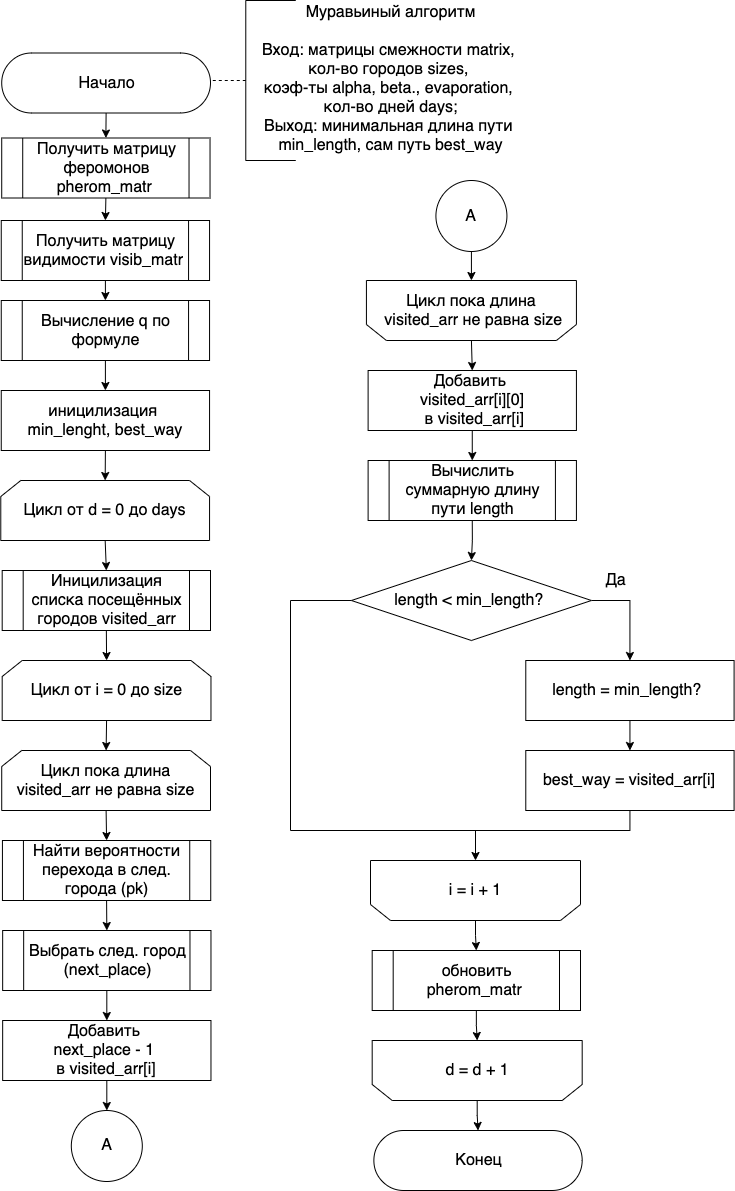
\includegraphics[scale=0.55]{img/ant_alg_scheme.png}
	\caption{Схема муравьиного алгоритма}
	\label{fig:ant_alg_scheme}
\end{figure}

\clearpage

\begin{figure}[h]
	\centering
	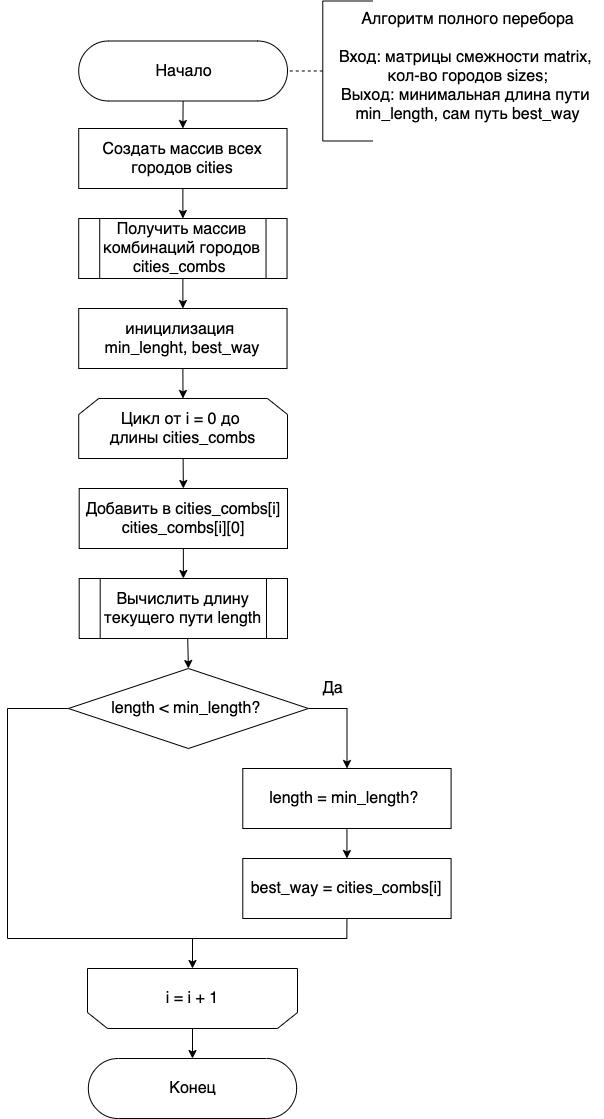
\includegraphics[scale=0.6]{img/full_comb_alg_scheme.png}
	\caption{Схема алгоритма полного перебора}
	\label{fig:full_comb_alg_scheme}
\end{figure}

\clearpage

\section{Классы эквивалентности}

Выделенные классы эквивалентности для тестирования:

\begin{itemize}
	\item коэффицент $\alpha$ <= 0;
	\item коэффицент $\alpha$ не является числом;
	\item коэффицент $\beta$ <= 0;
	\item коэффицент $\beta$ не является числом;
	\item коэффицент $evaporation$ <= 0;
	\item коэффицент $evaporation$ не является числом;
	\item номер команды < 0 или > 5;
	\item номер команды не является целым числом;
	\item корректный ввод всех параметров;
\end{itemize}

\section{Описание используемых типов данных}

При реализации алгоритмов будут использованы следующие структуры данных:

\begin{itemize}
	\item размер матрицы смежности - целое число типа $int$;
	\item матрица смежности - матрица, элементы которой имеют тип $int$;
	\item коэффиценты $\alpha$, $\beta$, $evaporation$ - действительные числа типа $float$;
	\item название файла - строка типа $str$.
\end{itemize}

\clearpage

\section{Структура ПО}

ПО будет состоять из следующих модулей:

\begin{itemize}
	\item $main.py$ -- файл, содержащий функцию $main$;
	\item $generate.py$ -- файл, содержащий функцию для генирации матриц;
    \item $ant\_algorythm.py$ -- файл, в котором содержатся функции муравьиного алгоритма для решения задачи коммивояжера;
    \item $full\_combinations.py$ -- файл, в котором содержатся функции алгоритма полного перебора для решения задачи коммивояжера;
    \item $parametrization.py$ -- файл, содержащий функцию параметризации для муравьиного алгоритма;
    \item $compare\_time.py$ -- файл, в котором содержатся функции для замера времени работы алгоритмов и построения графика зависимоти времени выполнения от размера матрицы;
    \item $read\_print.py$ -- файл, в котором содержатся функции ввода вывода данных;
    \item $color.py$ -- файл, который содержит переменные типа $string$ для цветного вывода результата работы программы в консоль.
\end{itemize}

\section{Вывод}

В данном разделе на основе теоретических данных были построены схемы требуемых алгоритмов решения задачи коммивояжера (муравьиного алгоритма и алгоритма полного перебора), выбраны используемые типы данных, выделены классы эквивалентности для тестирования, а также была описана структура ПО.

\clearpage





\chapter{Технологическая часть}

В данном разделе будут приведены средства реализации, листинги кода, а также функциональные тесты.


\section{Средства реализации}

В данной работе для реализации был выбран язык программирования $Python$ [4]. Выбор обсуловлен наличием опыта работы с ним. Время работы было замерено с помощью функции \textit{process\_time} из библиотеки $time$ [5].

\section{Листинги кода}

В листингах \ref{lst:ant_alg} - \ref{lst:ant_alg} представлены функции для конвейерного и ленейного алгоритмов обработки матриц.

\begin{center}
\captionsetup{justification=raggedright,singlelinecheck=off}
\begin{lstlisting}[label=lst:full_combinations_alg,caption=Алгоритм полного перебора]
def full_combinations_alg(matrix, size):

	cities = np.arange(size)
	cities_combs = []

	for combination in it.permutations(cities):
		cities_combs.append(list(combination))

	best_way = []
	min_length = float("inf")

	for i in range(len(cities_combs)):
		cities_combs[i].append(cities_combs[i][0])

		length = calc_length(matrix, size, cities_combs[i])

		if length < min_length:
			min_length = length
			best_way = cities_combs[i]

	return min_length, best_way
\end{lstlisting}
\end{center}	

\clearpage

\begin{center}
\captionsetup{justification=raggedright,singlelinecheck=off}
\begin{lstlisting}[label=lst:ant_alg,caption=Муравьиный алгоритм]
def ant_alg(matrix, size, alpha, beta, evaporation, days):

	pherom_matr = get_pherom_matr(size)
	visib_matr = get_visib_matr(matrix, size)

	q = calc_q(matrix, size)

	best_way = []
	min_length = float("inf")

	for _ in range(days):
		visited_arr = get_visited_places(np.arange(size), size)

		for i in range(size):
			while (len(visited_arr[i]) != size):
				pk = search_probability(pherom_matr, visib_matr, visited_arr, size, i, alpha, beta)  
				next_place = choose_next_place(pk)

				visited_arr[i].append(next_place - 1)

			visited_arr[i].append(visited_arr[i][0])
			
			length = calc_length(matrix, size, visited_arr[i]) 

			if length < min_length:
				min_length = length
				best_way = visited_arr[i]

		pherom_matr = update_pherom_matr(matrix, size, visited_arr, pherom_matr, q, evaporation)

	return min_length, best_way
\end{lstlisting}
\end{center}

\clearpage

\begin{center}
\captionsetup{justification=raggedright,singlelinecheck=off}
\begin{lstlisting}[label=lst:update_pherom_matr,caption=Функция для обновления феромонов]
def update_pherom_matr(matrix, size, visited_arr, pherom_matr, q, evaporation):

	ants = size

	for i in range(size):
		for j in range(size):
			delta_pherom_matr = 0

			for ant in range(ants):
				length = calc_length(matrix, size, visited_arr[ant])
				delta_pherom_matr += q / length

			pherom_matr[i][j] *= (1 - evaporation)
			pherom_matr[i][j] += delta_pherom_matr

			if pherom_matr[i][j] < MIN_PHEROMONE:
			pherom_matr[i][j] = MIN_PHEROMONE

	return pherom_matr
\end{lstlisting}
\end{center}	

\begin{center}
\captionsetup{justification=raggedright,singlelinecheck=off}
\begin{lstlisting}[label=lst:search_probability,caption=Функция для нахождения вероятней перехода в каждый из городов]
def search_probability(pherom_matr, visib_matr, visited_arr, size, ant, alpha, beta):
    pk = [0] * size

    for i in range(size):
        if i not in visited_arr[ant]:
            ant_i = visited_arr[ant][-1]

            pk[i] = pow(pherom_matr[ant_i][i], alpha) * \
                    pow(visib_matr[ant_i][i], beta)
        else:
            pk[i] = 0

    pk_sum = sum(pk)

    for i in range(size):
        pk[i] /= pk_sum  

    return pk
\end{lstlisting}
\end{center}

\clearpage

\begin{center}
\captionsetup{justification=raggedright,singlelinecheck=off}
\begin{lstlisting}[label=lst:choose_next_place,caption=Функция выбора следующего города]
def choose_next_place(pk):

    size = len(pk)
    numb = 0
    i = 0

    probability = random()

    while numb < probability and i < size:
        numb += pk[i]
        i += 1

    return i
\end{lstlisting}
\end{center}	

\begin{center}
\captionsetup{justification=raggedright,singlelinecheck=off}
\begin{lstlisting}[label=lst:calc_length,caption= Функция нахождения длины пути]
def calc_length(matrix, size, way):

    length = 0

    for i in range(size):
        beg_city = way[i]
        end_city = way[i + 1]

        length += matrix[beg_city][end_city]

    return length
\end{lstlisting}
\end{center}

\clearpage

\section{Функциональные тесты}

В таблице \ref{tbl:functional_test} приведены функциональные тесты для алгоритмов решения задачи коммивояжера (муравьиного алгоритма и алгоритма полного перебора). Все тесты пройдены успешно.

\begin{center}
\captionsetup{justification=raggedright,singlelinecheck=off}
\begin{longtable}[c]{|c|c|c|}
\caption{Функциональные тесты\label{tbl:functional_test}}
	\\ \hline
	Матрица смежности & Результат & Ожидаемый результат 
	\\ \hline
	$\begin{pmatrix}
		0 & 1 & 2\\
		1 & 0 & 3\\
		2 & 3 & 0
	\end{pmatrix}$ & 6, [0, 1, 2, 0] & 6, [0, 1, 2, 0]
	\\ \hline
	$\begin{pmatrix}
		0 & 3 & 4 & 1\\
		3 & 0 & 1 & 1\\
		4 & 1 & 0 & 2\\
		1 & 1 & 2 & 0
	\end{pmatrix}$ & 7, [0, 1, 2, 3, 0] & 7, [0, 1, 2, 3, 0]
	\\ \hline
	$\begin{pmatrix}
		0 & 11 & 12 & 14 & 13\\
		11 & 0 & 15 & 10 & 10\\
		12 & 15 & 0 & 14 & 13\\
		14 & 10 & 14 & 0 & 10\\
		13 & 10 & 13 & 10 & 0\\
	\end{pmatrix}$ & 56, [0, 1, 3, 4, 2, 0] & 56, [0, 1, 3, 4, 2, 0]
	\\ \hline

\end{longtable}
\end{center}


\section{Вывод}

В данном разделе были разработаны алгоритмы решения задачи коммивояжера (муравьиный алгоритм и алгоритм полного перебора), проведено тестирование, описаны средства реализации.





\chapter{Исследовательская часть}

\section{Технические характеристики}

Технические характеристики устройства, на котором выполнялось тестирование представлены далее.

\begin{itemize}
    \item Операционная система: macOS 11.5.2. [6]
    \item Память: 8 GiB.
    \item Процессор: 2,3 GHz 4‑ядерный процессор Intel Core i5. [7]
\end{itemize}

При тестировании ноутбук был включен в сеть электропитания. Во время тестирования ноутбук был нагружен только встроенными приложениями окружения, а также системой тестирования.

\clearpage

\section{Демонстрация работы программы}

\img{220mm}{example}{Пример работы программы}

\clearpage

\section{Время выполнения алгоритмов}

Результаты замеров времени работы алгоритмов решения задачи коммивояжера представлены на рисунках 4.3 - 4.5. Замеры времени проводились в секундах и усреднялись для каждого набора одинаковых экспериментов.

\img{60mm}{time}{Замеры времени работы для муравьиного алгоритиа и алгоритма полного перебора}

\img{110mm}{graph}{Зависимость времени работы алгоритмов от размера матриц}

\clearpage

\section{Автоматическая параметризация}

Автоматическая параметризация была проведена на двух классах данных. Для проведение эксперимета были взяты матрицы размером 10x10. Муравьиный алгоритм был запущен для всех значений $\alpha, \rho \in (0, 1)$ с шагом 0.1.

В качестве эталонного значения был взят результат работы алгоритма полного перебора. 

Далее будут представлены матрицы смежности (матрица \ref{eq:kd1} для первого класса данных и \ref{eq:kd2} для второго), на которых происходила параметризация и таблицы с результами её выполнения.

\subsection{Класс данных 1}

В качестве первого класса данных была взята матрица смежности, в которой все значения незначительно отличаются друг от друга, находятся в диапазоне [1, 3].

\begin{equation}
    \label{eq:kd1}
	M_{1} = \begin{pmatrix}
		0 & 2 & 1 & 1 & 3 & 3 & 2 & 2 & 3 & 3 \\
		2 & 0 & 3 & 3 & 3 & 1 & 3 & 2 & 2 & 3 \\
		1 & 3 & 0 & 2 & 3 & 3 & 1 & 1 & 2 & 3 \\
		1 & 3 & 2 & 0 & 2 & 3 & 2 & 3 & 1 & 3 \\
		3 & 3 & 3 & 2 & 0 & 3 & 2 & 3 & 1 & 1 \\
		3 & 1 & 3 & 3 & 3 & 0 & 1 & 1 & 2 & 1 \\
		2 & 3 & 1 & 2 & 2 & 1 & 0 & 2 & 1 & 2 \\
		2 & 2 & 1 & 3 & 3 & 1 & 2 & 0 & 2 & 3 \\
		3 & 2 & 2 & 1 & 1 & 2 & 1 & 2 & 0 & 2 \\
		3 & 3 & 3 & 3 & 1 & 1 & 2 & 3 & 2 & 0 
	\end{pmatrix}
\end{equation}

\clearpage

\begin{center}
\captionsetup{justification=raggedright,singlelinecheck=off}
\begin{longtable}[c]{|c|c|c|c|c|c|}
\caption{Параметры для класса данных 1\label{tbl:table_kd1}}
	\\ \hline
	$\alpha$ & $\beta$ & $\rho$ & Дней & Результат & Ошибка 
	\\ \hline
	0.1 &  0.9 &  0.1 &   50 &    12 &     1 \\
	0.1 &  0.9 &  0.1 &  100 &    12 &     1 \\
	0.1 &  0.9 &  0.1 &  200 &    12 &     0 \\
   \hline
	0.1 &  0.9 &  0.2 &   50 &    12 &     0 \\
	0.1 &  0.9 &  0.2 &  100 &    12 &     0 \\
	0.1 &  0.9 &  0.2 &  200 &    12 &     0 \\
   \hline
	0.1 &  0.9 &  0.3 &   50 &    12 &     1 \\
	0.1 &  0.9 &  0.3 &  100 &    12 &     1 \\
	0.1 &  0.9 &  0.3 &  200 &    12 &     0 \\
   \hline
	0.1 &  0.9 &  0.4 &   50 &    12 &     1 \\
	0.1 &  0.9 &  0.4 &  100 &    12 &     0 \\
	0.1 &  0.9 &  0.4 &  200 &    12 &     0 \\
   \hline
	0.1 &  0.9 &  0.5 &   50 &    12 &     0 \\
	0.1 &  0.9 &  0.5 &  100 &    12 &     0 \\
	0.1 &  0.9 &  0.5 &  200 &    12 &     0 \\
   \hline
	0.1 &  0.9 &  0.6 &   50 &    12 &     1 \\
	0.1 &  0.9 &  0.6 &  100 &    12 &     1 \\
	0.1 &  0.9 &  0.6 &  200 &    12 &     0 \\
   \hline
	0.1 &  0.9 &  0.7 &   50 &    12 &     1 \\
	0.1 &  0.9 &  0.7 &  100 &    12 &     0 \\
	0.1 &  0.9 &  0.7 &  200 &    12 &     0 \\
   \hline
	0.1 &  0.9 &  0.8 &   50 &    12 &     1 \\
	0.1 &  0.9 &  0.8 &  100 &    12 &     0 \\
	0.1 &  0.9 &  0.8 &  200 &    12 &     0 \\
   \hline
	0.2 &  0.8 &  0.1 &   50 &    12 &     0 \\
	0.2 &  0.8 &  0.1 &  100 &    12 &     1 \\
	0.2 &  0.8 &  0.1 &  200 &    12 &     1 \\
   \hline
	0.2 &  0.8 &  0.2 &   50 &    12 &     1 \\
	0.2 &  0.8 &  0.2 &  100 &    12 &     0 \\
	0.2 &  0.8 &  0.2 &  200 &    12 &     0 \\
   \hline
	0.2 &  0.8 &  0.3 &   50 &    12 &     0 \\
	0.2 &  0.8 &  0.3 &  100 &    12 &     0 \\
	0.2 &  0.8 &  0.3 &  200 &    12 &     0 \\
   \hline
	0.2 &  0.8 &  0.4 &   50 &    12 &     0 \\
	0.2 &  0.8 &  0.4 &  100 &    12 &     0 \\
	0.2 &  0.8 &  0.4 &  200 &    12 &     0 \\
   \hline
	0.2 &  0.8 &  0.5 &   50 &    12 &     1 \\
	0.2 &  0.8 &  0.5 &  100 &    12 &     0 \\
	0.2 &  0.8 &  0.5 &  200 &    12 &     1 \\
   \hline
	0.2 &  0.8 &  0.6 &   50 &    12 &     0 \\
	0.2 &  0.8 &  0.6 &  100 &    12 &     0 \\
	0.2 &  0.8 &  0.6 &  200 &    12 &     0 \\
   \hline
	0.2 &  0.8 &  0.7 &   50 &    12 &     1 \\
	0.2 &  0.8 &  0.7 &  100 &    12 &     1 \\
	0.2 &  0.8 &  0.7 &  200 &    12 &     0 \\
   \hline
	0.2 &  0.8 &  0.8 &   50 &    12 &     1 \\
	0.2 &  0.8 &  0.8 &  100 &    12 &     0 \\
	0.2 &  0.8 &  0.8 &  200 &    12 &     0 \\
   \hline
	0.3 &  0.7 &  0.1 &   50 &    12 &     0 \\
	0.3 &  0.7 &  0.1 &  100 &    12 &     1 \\
	0.3 &  0.7 &  0.1 &  200 &    12 &     1 \\
   \hline
	0.3 &  0.7 &  0.2 &   50 &    12 &     0 \\
	0.3 &  0.7 &  0.2 &  100 &    12 &     0 \\
	0.3 &  0.7 &  0.2 &  200 &    12 &     0 \\
   \hline
	0.3 &  0.7 &  0.3 &   50 &    12 &     1 \\
	0.3 &  0.7 &  0.3 &  100 &    12 &     1 \\
	0.3 &  0.7 &  0.3 &  200 &    12 &     0 \\
   \hline
	0.3 &  0.7 &  0.4 &   50 &    12 &     1 \\
	0.3 &  0.7 &  0.4 &  100 &    12 &     0 \\
	0.3 &  0.7 &  0.4 &  200 &    12 &     1 \\
   \hline
	0.3 &  0.7 &  0.5 &   50 &    12 &     0 \\
	0.3 &  0.7 &  0.5 &  100 &    12 &     1 \\
	0.3 &  0.7 &  0.5 &  200 &    12 &     0 \\
   \hline
	0.3 &  0.7 &  0.6 &   50 &    12 &     2 \\
	0.3 &  0.7 &  0.6 &  100 &    12 &     1 \\
	0.3 &  0.7 &  0.6 &  200 &    12 &     1 \\
   \hline
	0.3 &  0.7 &  0.7 &   50 &    12 &     1 \\
	0.3 &  0.7 &  0.7 &  100 &    12 &     1 \\
	0.3 &  0.7 &  0.7 &  200 &    12 &     0 \\
   \hline
	0.3 &  0.7 &  0.8 &   50 &    12 &     1 \\
	0.3 &  0.7 &  0.8 &  100 &    12 &     1 \\
	0.3 &  0.7 &  0.8 &  200 &    12 &     1 \\
   \hline
	0.4 &  0.6 &  0.1 &   50 &    12 &     1 \\
	0.4 &  0.6 &  0.1 &  100 &    12 &     0 \\
	0.4 &  0.6 &  0.1 &  200 &    12 &     0 \\
   \hline
	0.4 &  0.6 &  0.2 &   50 &    12 &     1 \\
	0.4 &  0.6 &  0.2 &  100 &    12 &     0 \\
	0.4 &  0.6 &  0.2 &  200 &    12 &     1 \\
   \hline
	0.4 &  0.6 &  0.3 &   50 &    12 &     0 \\
	0.4 &  0.6 &  0.3 &  100 &    12 &     0 \\
	0.4 &  0.6 &  0.3 &  200 &    12 &     1 \\
   \hline
	0.4 &  0.6 &  0.4 &   50 &    12 &     1 \\
	0.4 &  0.6 &  0.4 &  100 &    12 &     0 \\
	0.4 &  0.6 &  0.4 &  200 &    12 &     0 \\
   \hline
	0.4 &  0.6 &  0.5 &   50 &    12 &     1 \\
	0.4 &  0.6 &  0.5 &  100 &    12 &     1 \\
	0.4 &  0.6 &  0.5 &  200 &    12 &     0 \\
   \hline
	0.4 &  0.6 &  0.6 &   50 &    12 &     0 \\
	0.4 &  0.6 &  0.6 &  100 &    12 &     1 \\
	0.4 &  0.6 &  0.6 &  200 &    12 &     0 \\
   \hline
	0.4 &  0.6 &  0.7 &   50 &    12 &     2 \\
	0.4 &  0.6 &  0.7 &  100 &    12 &     1 \\
	0.4 &  0.6 &  0.7 &  200 &    12 &     0 \\
   \hline
	0.4 &  0.6 &  0.8 &   50 &    12 &     1 \\
	0.4 &  0.6 &  0.8 &  100 &    12 &     1 \\
	0.4 &  0.6 &  0.8 &  200 &    12 &     0 \\
   \hline
	0.5 &  0.5 &  0.1 &   50 &    12 &     2 \\
	0.5 &  0.5 &  0.1 &  100 &    12 &     0 \\
	0.5 &  0.5 &  0.1 &  200 &    12 &     1 \\
   \hline
	0.5 &  0.5 &  0.2 &   50 &    12 &     1 \\
	0.5 &  0.5 &  0.2 &  100 &    12 &     0 \\
	0.5 &  0.5 &  0.2 &  200 &    12 &     1 \\
   \hline
	0.5 &  0.5 &  0.3 &   50 &    12 &     2 \\
	0.5 &  0.5 &  0.3 &  100 &    12 &     1 \\
	0.5 &  0.5 &  0.3 &  200 &    12 &     1 \\
   \hline
	0.5 &  0.5 &  0.4 &   50 &    12 &     2 \\
	0.5 &  0.5 &  0.4 &  100 &    12 &     1 \\
	0.5 &  0.5 &  0.4 &  200 &    12 &     0 \\
   \hline
	0.5 &  0.5 &  0.5 &   50 &    12 &     2 \\
	0.5 &  0.5 &  0.5 &  100 &    12 &     1 \\
	0.5 &  0.5 &  0.5 &  200 &    12 &     1 \\
   \hline
	0.5 &  0.5 &  0.6 &   50 &    12 &     2 \\
	0.5 &  0.5 &  0.6 &  100 &    12 &     1 \\
	0.5 &  0.5 &  0.6 &  200 &    12 &     1 \\
   \hline
	0.5 &  0.5 &  0.7 &   50 &    12 &     2 \\
	0.5 &  0.5 &  0.7 &  100 &    12 &     0 \\
	0.5 &  0.5 &  0.7 &  200 &    12 &     0 \\
   \hline
	0.5 &  0.5 &  0.8 &   50 &    12 &     1 \\
	0.5 &  0.5 &  0.8 &  100 &    12 &     1 \\
	0.5 &  0.5 &  0.8 &  200 &    12 &     1 \\
   \hline
	0.6 &  0.4 &  0.1 &   50 &    12 &     1 \\
	0.6 &  0.4 &  0.1 &  100 &    12 &     0 \\
	0.6 &  0.4 &  0.1 &  200 &    12 &     1 \\
   \hline
	0.6 &  0.4 &  0.2 &   50 &    12 &     2 \\
	0.6 &  0.4 &  0.2 &  100 &    12 &     1 \\
	0.6 &  0.4 &  0.2 &  200 &    12 &     1 \\
   \hline
	0.6 &  0.4 &  0.3 &   50 &    12 &     1 \\
	0.6 &  0.4 &  0.3 &  100 &    12 &     2 \\
	0.6 &  0.4 &  0.3 &  200 &    12 &     1 \\
   \hline
	0.6 &  0.4 &  0.4 &   50 &    12 &     1 \\
	0.6 &  0.4 &  0.4 &  100 &    12 &     0 \\
	0.6 &  0.4 &  0.4 &  200 &    12 &     0 \\
   \hline
	0.6 &  0.4 &  0.5 &   50 &    12 &     1 \\
	0.6 &  0.4 &  0.5 &  100 &    12 &     1 \\
	0.6 &  0.4 &  0.5 &  200 &    12 &     1 \\
   \hline
	0.6 &  0.4 &  0.6 &   50 &    12 &     1 \\
	0.6 &  0.4 &  0.6 &  100 &    12 &     1 \\
	0.6 &  0.4 &  0.6 &  200 &    12 &     1 \\
   \hline
	0.6 &  0.4 &  0.7 &   50 &    12 &     1 \\
	0.6 &  0.4 &  0.7 &  100 &    12 &     1 \\
	0.6 &  0.4 &  0.7 &  200 &    12 &     1 \\
   \hline
	0.6 &  0.4 &  0.8 &   50 &    12 &     1 \\
	0.6 &  0.4 &  0.8 &  100 &    12 &     2 \\
	0.6 &  0.4 &  0.8 &  200 &    12 &     1 \\
   \hline
	0.7 &  0.3 &  0.1 &   50 &    12 &     2 \\
	0.7 &  0.3 &  0.1 &  100 &    12 &     1 \\
	0.7 &  0.3 &  0.1 &  200 &    12 &     1 \\
   \hline
	0.7 &  0.3 &  0.2 &   50 &    12 &     1 \\
	0.7 &  0.3 &  0.2 &  100 &    12 &     1 \\
	0.7 &  0.3 &  0.2 &  200 &    12 &     1 \\
   \hline
	0.7 &  0.3 &  0.3 &   50 &    12 &     2 \\
	0.7 &  0.3 &  0.3 &  100 &    12 &     1 \\
	0.7 &  0.3 &  0.3 &  200 &    12 &     1 \\
   \hline
	0.7 &  0.3 &  0.4 &   50 &    12 &     2 \\
	0.7 &  0.3 &  0.4 &  100 &    12 &     1 \\
	0.7 &  0.3 &  0.4 &  200 &    12 &     0 \\
   \hline
	0.7 &  0.3 &  0.5 &   50 &    12 &     2 \\
	0.7 &  0.3 &  0.5 &  100 &    12 &     1 \\
	0.7 &  0.3 &  0.5 &  200 &    12 &     1 \\
   \hline
	0.7 &  0.3 &  0.6 &   50 &    12 &     3 \\
	0.7 &  0.3 &  0.6 &  100 &    12 &     2 \\
	0.7 &  0.3 &  0.6 &  200 &    12 &     1 \\
   \hline
	0.7 &  0.3 &  0.7 &   50 &    12 &     2 \\
	0.7 &  0.3 &  0.7 &  100 &    12 &     2 \\
	0.7 &  0.3 &  0.7 &  200 &    12 &     1 \\
   \hline
	0.7 &  0.3 &  0.8 &   50 &    12 &     2 \\
	0.7 &  0.3 &  0.8 &  100 &    12 &     1 \\
	0.7 &  0.3 &  0.8 &  200 &    12 &     0 \\
   \hline
	0.8 &  0.2 &  0.1 &   50 &    12 &     1 \\
	0.8 &  0.2 &  0.1 &  100 &    12 &     2 \\
	0.8 &  0.2 &  0.1 &  200 &    12 &     1 \\
   \hline
	0.8 &  0.2 &  0.2 &   50 &    12 &     2 \\
	0.8 &  0.2 &  0.2 &  100 &    12 &     2 \\
	0.8 &  0.2 &  0.2 &  200 &    12 &     1 \\
   \hline
	0.8 &  0.2 &  0.3 &   50 &    12 &     1 \\
	0.8 &  0.2 &  0.3 &  100 &    12 &     2 \\
	0.8 &  0.2 &  0.3 &  200 &    12 &     1 \\
   \hline
	0.8 &  0.2 &  0.4 &   50 &    12 &     1 \\
	0.8 &  0.2 &  0.4 &  100 &    12 &     2 \\
	0.8 &  0.2 &  0.4 &  200 &    12 &     1 \\
   \hline
	0.8 &  0.2 &  0.5 &   50 &    12 &     2 \\
	0.8 &  0.2 &  0.5 &  100 &    12 &     1 \\
	0.8 &  0.2 &  0.5 &  200 &    12 &     0 \\
   \hline
	0.8 &  0.2 &  0.6 &   50 &    12 &     2 \\
	0.8 &  0.2 &  0.6 &  100 &    12 &     1 \\
	0.8 &  0.2 &  0.6 &  200 &    12 &     0 \\
   \hline
	0.8 &  0.2 &  0.7 &   50 &    12 &     2 \\
	0.8 &  0.2 &  0.7 &  100 &    12 &     2 \\
	0.8 &  0.2 &  0.7 &  200 &    12 &     2 \\
   \hline
	0.8 &  0.2 &  0.8 &   50 &    12 &     0 \\
	0.8 &  0.2 &  0.8 &  100 &    12 &     1 \\
	0.8 &  0.2 &  0.8 &  200 &    12 &     1 \\
   \hline
	0.9 &  0.1 &  0.1 &   50 &    12 &     2 \\
	0.9 &  0.1 &  0.1 &  100 &    12 &     1 \\
	0.9 &  0.1 &  0.1 &  200 &    12 &     2 \\
   \hline
	0.9 &  0.1 &  0.2 &   50 &    12 &     2 \\
	0.9 &  0.1 &  0.2 &  100 &    12 &     1 \\
	0.9 &  0.1 &  0.2 &  200 &    12 &     0 \\
   \hline
	0.9 &  0.1 &  0.3 &   50 &    12 &     3 \\
	0.9 &  0.1 &  0.3 &  100 &    12 &     1 \\
	0.9 &  0.1 &  0.3 &  200 &    12 &     1 \\
   \hline
	0.9 &  0.1 &  0.4 &   50 &    12 &     3 \\
	0.9 &  0.1 &  0.4 &  100 &    12 &     1 \\
	0.9 &  0.1 &  0.4 &  200 &    12 &     2 \\
   \hline
	0.9 &  0.1 &  0.5 &   50 &    12 &     2 \\
	0.9 &  0.1 &  0.5 &  100 &    12 &     2 \\
	0.9 &  0.1 &  0.5 &  200 &    12 &     2 \\
   \hline
	0.9 &  0.1 &  0.6 &   50 &    12 &     2 \\
	0.9 &  0.1 &  0.6 &  100 &    12 &     2 \\
	0.9 &  0.1 &  0.6 &  200 &    12 &     1 \\
   \hline
	0.9 &  0.1 &  0.7 &   50 &    12 &     2 \\
	0.9 &  0.1 &  0.7 &  100 &    12 &     1 \\
	0.9 &  0.1 &  0.7 &  200 &    12 &     1 \\
   \hline
	0.9 &  0.1 &  0.8 &   50 &    12 &     2 \\
	0.9 &  0.1 &  0.8 &  100 &    12 &     2 \\
	0.9 &  0.1 &  0.8 &  200 &    12 &     1 \\
   \hline
\end{longtable}
\end{center}

\clearpage

\subsection{Класс данных 2}

В качестве второго класса данных была взята матрица смежности, в которой все значения отличюатся на большое значение друг от друга, находятся в диапазоне [1, 1000].

\begin{equation}
    \label{eq:kd2}
	M_{2} = \begin{pmatrix}
		0 & 157 & 611 & 117 & 341 & 452 & 579 & 773 & 370 & 343 \\
		157 & 0 & 170 & 696 & 238 & 669 & 302 & 633 & 111 & 427 \\
		611 & 170 & 0 & 95 & 829 & 14 & 661 & 118 & 871 & 754 \\
		117 & 696 & 95 & 0 & 37 & 535 & 308 & 996 & 419 & 456 \\
		341 & 238 & 829 & 37 & 0 & 854 & 454 & 908 & 806 & 455 \\
		452 & 669 & 14 & 535 & 854 & 0 & 646 & 262 & 400 & 799 \\
		579 & 302 & 661 & 308 & 454 & 646 & 0 & 139 & 982 & 423 \\
		773 & 633 & 118 & 996 & 908 & 262 & 139 & 0 & 887 & 59 \\
		370 & 111 & 871 & 419 & 806 & 400 & 982 & 887 & 0 & 578 \\
		343 & 427 & 754 & 456 & 455 & 799 & 423 & 59 & 578 & 0 
	\end{pmatrix}
\end{equation}


\begin{center}
\captionsetup{justification=raggedright,singlelinecheck=off}
\begin{longtable}[c]{|c|c|c|c|c|c|}
\caption{Параметры для класса данных 2\label{tbl:table_kd2}}
		\\ \hline
		$\alpha$ & $\beta$ & $\rho$ & Дней & Результат & Ошибка 
		\\ \hline
		0.1 &  0.9 &  0.1 &   50 &  1809 &     0 \\
		0.1 &  0.9 &  0.1 &  100 &  1809 &     0 \\
		0.1 &  0.9 &  0.1 &  200 &  1809 &     0 \\
	   \hline
		0.1 &  0.9 &  0.2 &   50 &  1809 &     0 \\
		0.1 &  0.9 &  0.2 &  100 &  1809 &    32 \\
		0.1 &  0.9 &  0.2 &  200 &  1809 &    32 \\
	   \hline
		0.1 &  0.9 &  0.3 &   50 &  1809 &     0 \\
		0.1 &  0.9 &  0.3 &  100 &  1809 &     0 \\
		0.1 &  0.9 &  0.3 &  200 &  1809 &    81 \\
	   \hline
		0.1 &  0.9 &  0.4 &   50 &  1809 &    32 \\
		0.1 &  0.9 &  0.4 &  100 &  1809 &     0 \\
		0.1 &  0.9 &  0.4 &  200 &  1809 &     0 \\
	   \hline
		0.1 &  0.9 &  0.5 &   50 &  1809 &    32 \\
		0.1 &  0.9 &  0.5 &  100 &  1809 &     0 \\
		0.1 &  0.9 &  0.5 &  200 &  1809 &     0 \\
	   \hline
		0.1 &  0.9 &  0.6 &   50 &  1809 &     0 \\
		0.1 &  0.9 &  0.6 &  100 &  1809 &     0 \\
		0.1 &  0.9 &  0.6 &  200 &  1809 &     0 \\
	   \hline
		0.1 &  0.9 &  0.7 &   50 &  1809 &   205 \\
		0.1 &  0.9 &  0.7 &  100 &  1809 &    32 \\
		0.1 &  0.9 &  0.7 &  200 &  1809 &     0 \\
	   \hline
		0.1 &  0.9 &  0.8 &   50 &  1809 &     0 \\
		0.1 &  0.9 &  0.8 &  100 &  1809 &     0 \\
		0.1 &  0.9 &  0.8 &  200 &  1809 &     0 \\
	   \hline
		0.2 &  0.8 &  0.1 &   50 &  1809 &     0 \\
		0.2 &  0.8 &  0.1 &  100 &  1809 &    32 \\
		0.2 &  0.8 &  0.1 &  200 &  1809 &     0 \\
	   \hline
		0.2 &  0.8 &  0.2 &   50 &  1809 &   146 \\
		0.2 &  0.8 &  0.2 &  100 &  1809 &     0 \\
		0.2 &  0.8 &  0.2 &  200 &  1809 &     0 \\
	   \hline
		0.2 &  0.8 &  0.3 &   50 &  1809 &    32 \\
		0.2 &  0.8 &  0.3 &  100 &  1809 &     0 \\
		0.2 &  0.8 &  0.3 &  200 &  1809 &     0 \\
	   \hline
		0.2 &  0.8 &  0.4 &   50 &  1809 &    81 \\
		0.2 &  0.8 &  0.4 &  100 &  1809 &    32 \\
		0.2 &  0.8 &  0.4 &  200 &  1809 &     0 \\
	   \hline
		0.2 &  0.8 &  0.5 &   50 &  1809 &     0 \\
		0.2 &  0.8 &  0.5 &  100 &  1809 &     0 \\
		0.2 &  0.8 &  0.5 &  200 &  1809 &     0 \\
	   \hline
		0.2 &  0.8 &  0.6 &   50 &  1809 &    32 \\
		0.2 &  0.8 &  0.6 &  100 &  1809 &    32 \\
		0.2 &  0.8 &  0.6 &  200 &  1809 &     0 \\
	   \hline
		0.2 &  0.8 &  0.7 &   50 &  1809 &    32 \\
		0.2 &  0.8 &  0.7 &  100 &  1809 &     0 \\
		0.2 &  0.8 &  0.7 &  200 &  1809 &     0 \\
	   \hline
		0.2 &  0.8 &  0.8 &   50 &  1809 &   162 \\
		0.2 &  0.8 &  0.8 &  100 &  1809 &     0 \\
		0.2 &  0.8 &  0.8 &  200 &  1809 &     0 \\
	   \hline
		0.3 &  0.7 &  0.1 &   50 &  1809 &    81 \\
		0.3 &  0.7 &  0.1 &  100 &  1809 &     0 \\
		0.3 &  0.7 &  0.1 &  200 &  1809 &    32 \\
	   \hline
		0.3 &  0.7 &  0.2 &   50 &  1809 &   131 \\
		0.3 &  0.7 &  0.2 &  100 &  1809 &     0 \\
		0.3 &  0.7 &  0.2 &  200 &  1809 &     0 \\
	   \hline
		0.3 &  0.7 &  0.3 &   50 &  1809 &    32 \\
		0.3 &  0.7 &  0.3 &  100 &  1809 &     0 \\
		0.3 &  0.7 &  0.3 &  200 &  1809 &     0 \\
	   \hline
		0.3 &  0.7 &  0.4 &   50 &  1809 &     0 \\
		0.3 &  0.7 &  0.4 &  100 &  1809 &     0 \\
		0.3 &  0.7 &  0.4 &  200 &  1809 &     0 \\
	   \hline
		0.3 &  0.7 &  0.5 &   50 &  1809 &   208 \\
		0.3 &  0.7 &  0.5 &  100 &  1809 &    32 \\
		0.3 &  0.7 &  0.5 &  200 &  1809 &     0 \\
	   \hline
		0.3 &  0.7 &  0.6 &   50 &  1809 &   131 \\
		0.3 &  0.7 &  0.6 &  100 &  1809 &    32 \\
		0.3 &  0.7 &  0.6 &  200 &  1809 &     0 \\
	   \hline
		0.3 &  0.7 &  0.7 &   50 &  1809 &    32 \\
		0.3 &  0.7 &  0.7 &  100 &  1809 &     0 \\
		0.3 &  0.7 &  0.7 &  200 &  1809 &     0 \\
	   \hline
		0.3 &  0.7 &  0.8 &   50 &  1809 &   131 \\
		0.3 &  0.7 &  0.8 &  100 &  1809 &     0 \\
		0.3 &  0.7 &  0.8 &  200 &  1809 &    32 \\
	   \hline
		0.4 &  0.6 &  0.1 &   50 &  1809 &    81 \\
		0.4 &  0.6 &  0.1 &  100 &  1809 &     0 \\
		0.4 &  0.6 &  0.1 &  200 &  1809 &     0 \\
	   \hline
		0.4 &  0.6 &  0.2 &   50 &  1809 &    81 \\
		0.4 &  0.6 &  0.2 &  100 &  1809 &   159 \\
		0.4 &  0.6 &  0.2 &  200 &  1809 &     0 \\
	   \hline
		0.4 &  0.6 &  0.3 &   50 &  1809 &     0 \\
		0.4 &  0.6 &  0.3 &  100 &  1809 &   161 \\
		0.4 &  0.6 &  0.3 &  200 &  1809 &     0 \\
	   \hline
		0.4 &  0.6 &  0.4 &   50 &  1809 &    32 \\
		0.4 &  0.6 &  0.4 &  100 &  1809 &   270 \\
		0.4 &  0.6 &  0.4 &  200 &  1809 &     0 \\
	   \hline
		0.4 &  0.6 &  0.5 &   50 &  1809 &   188 \\
		0.4 &  0.6 &  0.5 &  100 &  1809 &    32 \\
		0.4 &  0.6 &  0.5 &  200 &  1809 &     0 \\
	   \hline
		0.4 &  0.6 &  0.6 &   50 &  1809 &    81 \\
		0.4 &  0.6 &  0.6 &  100 &  1809 &    81 \\
		0.4 &  0.6 &  0.6 &  200 &  1809 &    32 \\
	   \hline
		0.4 &  0.6 &  0.7 &   50 &  1809 &    32 \\
		0.4 &  0.6 &  0.7 &  100 &  1809 &   188 \\
		0.4 &  0.6 &  0.7 &  200 &  1809 &    32 \\
	   \hline
		0.4 &  0.6 &  0.8 &   50 &  1809 &   378 \\
		0.4 &  0.6 &  0.8 &  100 &  1809 &   161 \\
		0.4 &  0.6 &  0.8 &  200 &  1809 &    32 \\
	   \hline
		0.5 &  0.5 &  0.1 &   50 &  1809 &   146 \\
		0.5 &  0.5 &  0.1 &  100 &  1809 &     0 \\
		0.5 &  0.5 &  0.1 &  200 &  1809 &    32 \\
	   \hline
		0.5 &  0.5 &  0.2 &   50 &  1809 &   273 \\
		0.5 &  0.5 &  0.2 &  100 &  1809 &     0 \\
		0.5 &  0.5 &  0.2 &  200 &  1809 &     0 \\
	   \hline
		0.5 &  0.5 &  0.3 &   50 &  1809 &   131 \\
		0.5 &  0.5 &  0.3 &  100 &  1809 &    32 \\
		0.5 &  0.5 &  0.3 &  200 &  1809 &     0 \\
	   \hline
		0.5 &  0.5 &  0.4 &   50 &  1809 &   205 \\
		0.5 &  0.5 &  0.4 &  100 &  1809 &     0 \\
		0.5 &  0.5 &  0.4 &  200 &  1809 &    32 \\
	   \hline
		0.5 &  0.5 &  0.5 &   50 &  1809 &   223 \\
		0.5 &  0.5 &  0.5 &  100 &  1809 &   159 \\
		0.5 &  0.5 &  0.5 &  200 &  1809 &     0 \\
	   \hline
		0.5 &  0.5 &  0.6 &   50 &  1809 &   224 \\
		0.5 &  0.5 &  0.6 &  100 &  1809 &    81 \\
		0.5 &  0.5 &  0.6 &  200 &  1809 &     0 \\
	   \hline
		0.5 &  0.5 &  0.7 &   50 &  1809 &   289 \\
		0.5 &  0.5 &  0.7 &  100 &  1809 &     0 \\
		0.5 &  0.5 &  0.7 &  200 &  1809 &     0 \\
	   \hline
		0.5 &  0.5 &  0.8 &   50 &  1809 &   205 \\
		0.5 &  0.5 &  0.8 &  100 &  1809 &    32 \\
		0.5 &  0.5 &  0.8 &  200 &  1809 &    81 \\
	   \hline
		0.6 &  0.4 &  0.1 &   50 &  1809 &   219 \\
		0.6 &  0.4 &  0.1 &  100 &  1809 &   131 \\
		0.6 &  0.4 &  0.1 &  200 &  1809 &     0 \\
	   \hline
		0.6 &  0.4 &  0.2 &   50 &  1809 &   162 \\
		0.6 &  0.4 &  0.2 &  100 &  1809 &   237 \\
		0.6 &  0.4 &  0.2 &  200 &  1809 &   146 \\
	   \hline
		0.6 &  0.4 &  0.3 &   50 &  1809 &    81 \\
		0.6 &  0.4 &  0.3 &  100 &  1809 &   161 \\
		0.6 &  0.4 &  0.3 &  200 &  1809 &     0 \\
	   \hline
		0.6 &  0.4 &  0.4 &   50 &  1809 &   269 \\
		0.6 &  0.4 &  0.4 &  100 &  1809 &    81 \\
		0.6 &  0.4 &  0.4 &  200 &  1809 &   131 \\
	   \hline
		0.6 &  0.4 &  0.5 &   50 &  1809 &   349 \\
		0.6 &  0.4 &  0.5 &  100 &  1809 &   219 \\
		0.6 &  0.4 &  0.5 &  200 &  1809 &     0 \\
	   \hline
		0.6 &  0.4 &  0.6 &   50 &  1809 &    32 \\
		0.6 &  0.4 &  0.6 &  100 &  1809 &     0 \\
		0.6 &  0.4 &  0.6 &  200 &  1809 &    81 \\
	   \hline
		0.6 &  0.4 &  0.7 &   50 &  1809 &     0 \\
		0.6 &  0.4 &  0.7 &  100 &  1809 &     0 \\
		0.6 &  0.4 &  0.7 &  200 &  1809 &    32 \\
	   \hline
		0.6 &  0.4 &  0.8 &   50 &  1809 &   224 \\
		0.6 &  0.4 &  0.8 &  100 &  1809 &   224 \\
		0.6 &  0.4 &  0.8 &  200 &  1809 &   131 \\
	   \hline
		0.7 &  0.3 &  0.1 &   50 &  1809 &   384 \\
		0.7 &  0.3 &  0.1 &  100 &  1809 &   146 \\
		0.7 &  0.3 &  0.1 &  200 &  1809 &   287 \\
	   \hline
		0.7 &  0.3 &  0.2 &   50 &  1809 &     0 \\
		0.7 &  0.3 &  0.2 &  100 &  1809 &   287 \\
		0.7 &  0.3 &  0.2 &  200 &  1809 &     0 \\
	   \hline
		0.7 &  0.3 &  0.3 &   50 &  1809 &   341 \\
		0.7 &  0.3 &  0.3 &  100 &  1809 &   237 \\
		0.7 &  0.3 &  0.3 &  200 &  1809 &   341 \\
	   \hline
		0.7 &  0.3 &  0.4 &   50 &  1809 &   239 \\
		0.7 &  0.3 &  0.4 &  100 &  1809 &   389 \\
		0.7 &  0.3 &  0.4 &  200 &  1809 &    81 \\
	   \hline
		0.7 &  0.3 &  0.5 &   50 &  1809 &   310 \\
		0.7 &  0.3 &  0.5 &  100 &  1809 &   353 \\
		0.7 &  0.3 &  0.5 &  200 &  1809 &     0 \\
	   \hline
		0.7 &  0.3 &  0.6 &   50 &  1809 &   313 \\
		0.7 &  0.3 &  0.6 &  100 &  1809 &   269 \\
		0.7 &  0.3 &  0.6 &  200 &  1809 &     0 \\
	   \hline
		0.7 &  0.3 &  0.7 &   50 &  1809 &   555 \\
		0.7 &  0.3 &  0.7 &  100 &  1809 &   225 \\
		0.7 &  0.3 &  0.7 &  200 &  1809 &     0 \\
	   \hline
		0.7 &  0.3 &  0.8 &   50 &  1809 &   470 \\
		0.7 &  0.3 &  0.8 &  100 &  1809 &   316 \\
		0.7 &  0.3 &  0.8 &  200 &  1809 &   243 \\
	   \hline
		0.8 &  0.2 &  0.1 &   50 &  1809 &    81 \\
		0.8 &  0.2 &  0.1 &  100 &  1809 &   569 \\
		0.8 &  0.2 &  0.1 &  200 &  1809 &   389 \\
	   \hline
		0.8 &  0.2 &  0.2 &   50 &  1809 &   162 \\
		0.8 &  0.2 &  0.2 &  100 &  1809 &   225 \\
		0.8 &  0.2 &  0.2 &  200 &  1809 &   348 \\
	   \hline
		0.8 &  0.2 &  0.3 &   50 &  1809 &   411 \\
		0.8 &  0.2 &  0.3 &  100 &  1809 &   450 \\
		0.8 &  0.2 &  0.3 &  200 &  1809 &   287 \\
	   \hline
		0.8 &  0.2 &  0.4 &   50 &  1809 &   539 \\
		0.8 &  0.2 &  0.4 &  100 &  1809 &    32 \\
		0.8 &  0.2 &  0.4 &  200 &  1809 &   237 \\
	   \hline
		0.8 &  0.2 &  0.5 &   50 &  1809 &   489 \\
		0.8 &  0.2 &  0.5 &  100 &  1809 &    32 \\
		0.8 &  0.2 &  0.5 &  200 &  1809 &   161 \\
	   \hline
		0.8 &  0.2 &  0.6 &   50 &  1809 &   208 \\
		0.8 &  0.2 &  0.6 &  100 &  1809 &   254 \\
		0.8 &  0.2 &  0.6 &  200 &  1809 &   146 \\
	   \hline
		0.8 &  0.2 &  0.7 &   50 &  1809 &   559 \\
		0.8 &  0.2 &  0.7 &  100 &  1809 &   161 \\
		0.8 &  0.2 &  0.7 &  200 &  1809 &   237 \\
	   \hline
		0.8 &  0.2 &  0.8 &   50 &  1809 &   161 \\
		0.8 &  0.2 &  0.8 &  100 &  1809 &   487 \\
		0.8 &  0.2 &  0.8 &  200 &  1809 &   188 \\
	   \hline
		0.9 &  0.1 &  0.1 &   50 &  1809 &   223 \\
		0.9 &  0.1 &  0.1 &  100 &  1809 &   146 \\
		0.9 &  0.1 &  0.1 &  200 &  1809 &   254 \\
	   \hline
		0.9 &  0.1 &  0.2 &   50 &  1809 &   433 \\
		0.9 &  0.1 &  0.2 &  100 &  1809 &   529 \\
		0.9 &  0.1 &  0.2 &  200 &  1809 &   413 \\
	   \hline
		0.9 &  0.1 &  0.3 &   50 &  1809 &   423 \\
		0.9 &  0.1 &  0.3 &  100 &  1809 &   458 \\
		0.9 &  0.1 &  0.3 &  200 &  1809 &   161 \\
	   \hline
		0.9 &  0.1 &  0.4 &   50 &  1809 &   482 \\
		0.9 &  0.1 &  0.4 &  100 &  1809 &   420 \\
		0.9 &  0.1 &  0.4 &  200 &  1809 &   387 \\
	   \hline
		0.9 &  0.1 &  0.5 &   50 &  1809 &   672 \\
		0.9 &  0.1 &  0.5 &  100 &  1809 &   319 \\
		0.9 &  0.1 &  0.5 &  200 &  1809 &    81 \\
	   \hline
		0.9 &  0.1 &  0.6 &   50 &  1809 &   322 \\
		0.9 &  0.1 &  0.6 &  100 &  1809 &   612 \\
		0.9 &  0.1 &  0.6 &  200 &  1809 &   146 \\
	   \hline
		0.9 &  0.1 &  0.7 &   50 &  1809 &   349 \\
		0.9 &  0.1 &  0.7 &  100 &  1809 &   467 \\
		0.9 &  0.1 &  0.7 &  200 &  1809 &   310 \\
	   \hline
		0.9 &  0.1 &  0.8 &   50 &  1809 &   237 \\
		0.9 &  0.1 &  0.8 &  100 &  1809 &   703 \\
		0.9 &  0.1 &  0.8 &  200 &  1809 &   387 \\
	   \hline	   
\end{longtable}
\end{center}

\clearpage

\section{Вывод}

В этом разделе были указаны технические характеристики машины, на которой происходило сравнение времени работы алгоритмов (муравьиного алгоритма и алгоритма полного перебора) решения задачи коммивояжера, также была рассмотрена автоматическая параметризация.

В результате замеров времени было установлено, что муравьиный алгоритм работает хуже алгоритма полного перебора на матрицах, размер которых меньше 9 (при размере 8 он работает хуже в 3.7 раза). Но при больших размерах муравьиный алгоритм существенно превосходит алгоритм полного перебора (на матрицах 9x9 он лучше в 2.1 раз, а на матрицах 10x10 уже в 15.4 раза). Во время проведения замеров времени кол-во дней для муравьиного алгоритма было взято 300.

На основе проведённой параметризации по двум классам данных можно сделать следующие выводы.

Для первого класса данных \ref{eq:kd1} лучше всего подходят следующие параметры:
\begin{itemize}
    \item $\alpha = 0.1, \beta = 0.9, \rho = 0.2, 0.5$;
    \item $\alpha = 0.2, \beta = 0.8, \rho = 0.3, 0.4, 06$;
    \item $\alpha = 0.3, \beta = 0.7, \rho = 0.2$;
\end{itemize}  

Для второго класса данных \ref{eq:kd2} лучше всего подходят следующие коэффиценты:
\begin{itemize}
    \item $\alpha = 0.1, \beta = 0.9, \rho = 0.1, 0.6, 0.8$;
    \item $\alpha = 0.2, \beta = 0.8, \rho = 0.5$;
    \item $\alpha = 0.3, \beta = 0.7, \rho = 0.4$;
\end{itemize}  

Таким образом, можно сделать вывод о том, что для лучшей работы муравьиного алгоритма на используемых классах данных (\ref{eq:kd1} и \ref{eq:kd2}) нужно использовать полученные коэффиценты.





\chapter*{Заключение}
\addcontentsline{toc}{chapter}{Заключение}

Было экспериментально подтверждено различие во временной эффективности муравьиного алгоритма и алгоритма полного перебора решения задачи коммивояжера. В результате исследований можно сделать вывод о том, что при матрицах большого размера (больше 9) стоит использовать муравьиный алгоритм решения задачи коммивояжера, а не алгоритм полного перебора (на матрице размером 10x10 он работает в 15.4 раза быстрее). Также было установлено по результатам параметризации на экспериментальных класса данных, что при коэффиценте $\alpha$ = 0.1, 0.2, 0.3 муравьиный алгоритм работает наилучшим образом.
\vspace{5mm}

В ходе выполнения данной лабораторной работы были решены следующие задачи:
\begin{itemize}
	\item изучены алгоритмы решения задачи коммивояжера (муравьиный алгоритм и алгоритм полного перебора);
	\item применены изученные основы для реализации описанных алгоритмов;
	\item произведен сравнительный анализ муравьиного алгоритма и алгорита полного перебора для решения задачи коммивояжера;
	\item экспериментально подтверждено различие во временнoй эффективности рассматриваемых алгоритмов при помощи разработанного программного обеспечения на материале замеров процессорного времени;
	\item проведена параметризация муравьиного алгоритма, которая показала лучшие наборы параметров для работы алгоритма на экспериментальных классах данных;
	\item описаны и обоснованы полученные результаты в отчете о выполненной лабораторной работе.
\end{itemize}

Поставленная цель была достигнута.





\begin{thebibliography}{5}
	\bibitem{bib1}
	Задача коммивояжёра [Электронный ресурс]. Режим доступа: \url{http://galyautdinov.ru/post/zadacha-kommivoyazhera} (дата обращения: 05.12.2021).
	\bibitem{bib2}
	Решаем задачу коммивояжёра простым перебором [Электронный ресурс]. Режим доступа: \url{https://thecode.media/path-js/} (дата обращения: 05.12.2021).
	\bibitem{bib3}
	Муравьиные алгоритмы [Электронный ресурс]. Режим доступа: \url{https://habr.com/ru/post/105302/} (дата обращения: 05.12.2021).
	\bibitem{bib4}
	Welcome to Python [Электронный ресурс]. Режим доступа: \url{https://www.python.org} (дата обращения: 18.10.2021).
	\bibitem{bib5}
	time — Time access and conversions [Электронный ресурс]. Режим доступа: \url{https://docs.python.org/3/library/time.html#functions} (дата обращения: 18.10.2021).
	\bibitem{bib6}
	macOS Monterey - Apple(RU) [Электронный ресурс]. Режим доступа: \url{https://www.apple.com/ru/macos/monterey/} (дата обращения: 14.10.2021).
	\bibitem{bib7}
	Intel [Электронный ресурс]. Режим доступа: \url{https://www.intel.ru/content/www/ru/ru/products/details/processors/core/i5.html} (дата обращения: 14.10.2021).
\end{thebibliography}

\addcontentsline{toc}{chapter}{Список литература}

\end{document}
